\section{Part 1: Modeling the Spread of Dandelions}

\subsection{Problem Analysis}
In this problem, the object of interest (a dandelion) is a living organism. This means the dandelion goes through standard phases during its life cycle: birth, growth, and death. The growth phase, where the dandelion transforms from seed to puffball, is based on factors that change over time, including temperature, light, and nutrients. Once a dandelion reaches puffball stage, those released seeds further contribute to the spread of dandelions.

\subsection {Assumptions}

\begin{table}[h]
\renewcommand{\arraystretch}{1.3}
    \begin{tabularx}{\textwidth}{lp{0.3\textwidth}X}
    \toprule
    \textbf{\#} & \textbf{Assumption} & {\centering \textbf{Justification}}  \\ \midrule
    
    \raggedright \nextassumption\label{assumption:1} & Dandelion seeds that land outside of the one-hectare plot of land will not be considered in our model.  & The problem statement refers to a dandelion adjacent to a plot of land, so we interpreted that as modeling the growth of dandelions on that plot of land only. \\

    \rowcolor{gray!15} \raggedright \nextassumption\label{assumption:2} & Dandelion seeds behave mostly independently (other than affecting other danelion seeds in their closest proximity). & This assumption allows us to develop an agent-based model to analyze the individual impacts of each seed and allow for much more easily adjustable hyperparameters. \\

    \raggedright \nextassumption\label{assumption:3} & Although consumers are considered on the plot of land, human disturbances do not occur.  & Because information is not provided about where the plot of land is located, we assume that although there could be consumers in the area, there are no humans that will cause a disturbance to the growth of the dandelions. \\

    \rowcolor{gray!15} \raggedright \nextassumption\label{assumption:4} & No natural disasters will occur during the 12 month period we are modeling.  & Because the probability of a natural disaster occurring is low (CITE), our model does not consider it. Additionally, our model of the climate on the plot of land includes more severe weather patterns that could occur throughout the year. \\

    \raggedright \nextassumption\label{assumption:5} & Nitrogen and potassium are the most important nutrients to consider in soil for the growth of dandelions.  & According to (CITE), higher potassium and nitrogen levels in the soil allow for increased seed germination and quicker growth CITE.\\

    \rowcolor{gray!15} \raggedright \nextassumption\label{assumption:6} & Wind is the only factor that spreads the seeds from a dandelion in its puffball stage.  & As stated previously, there are no human disturbances that could cause seeds to spread; therefore, the only other natural factor that can cause the seeds to spread is wind. \\ 
    \bottomrule
    \end{tabularx}
\end{table}

\subsection{Brief Overview}
As the problem begins with a single dandelion in the puffball stage, we begin our process by modeling the spread of the seeds of a dandelion. Afterward, we minimize the scope of the problem, focusing on each individual seed to model the independent growth of a seed. Once each seed matures into a puffball, we repeat the process.

To model the life cycles of many seeds, we developed a \textit{Seed Agent Model}, which considers land characteristics, such as wind, temperature, sunlight, and nutrients, to iterate through a germination and plant growth life cycle. Finally, the Seed Agent Model is applied to every seed in the motion process.

\subsection{Variables}

Our model presents a region-calibrated framework for various regions and climates to collect and modify our simulated model to their environment. Below is a table of variables outlining the core parameters of our model.

\begin{table}[h]
\renewcommand{\arraystretch}{1.3}
%p{0.8\linewidth
    \begin{tabularx}{\textwidth}{p{0.25\textwidth} lX}
    \toprule
    \textbf{Variable}           & \textbf{Symbol} & \textbf{Description}  \\ \midrule
    \raggedright Time Step & $t$  & Each time step is a day where \(t = 0\) is January 1 of a year. \\
    \rowcolor{gray!15}
    \raggedright Number of Moves & $N(t)$  & Number of moves a seed takes in movement process. \\
    Coordinate Shift & $\Delta x, \Delta y$    &  Change in \(x\) or \(y\) coordinate of a seed in every move.  \\
    \rowcolor{gray!15} \raggedright  Death Date & $D$               &  Time of death of a seed, sampled from Exponential distribution.  \\
    \raggedright Plant Growth & $G$ & The stage of growth of a dandelion plant between 0 and 1. \\
    \rowcolor{gray!15} \raggedright Temperature Index & $T_I$ & The index score of temperature where plants grow optimally in some particular range. \\
    \raggedright Light Index & $L_I$ & The index score of light levels where plants grow optimally in some particular range. \\
    \rowcolor{gray!15} \raggedright Nutrition Index & $N_I$ & The index score of soil nutrition where plants grow optimally in some particular soil conditions. \\
    \bottomrule
    \end{tabularx}
\end{table}

\subsection{The Way Of The Wind: A Seed Dispersal Process}

We first identified the primary contributing factor of dandelion seed movement to be the wind \cite{wang_separating_2021}. Thus, to model the spread of dandelion seeds, we use a Brownian Motion Process. Brownian Motion stochastic processes are often utilized to model the stochastic, or randomness within a probabilistic system, movement of particles in a particular medium, such as seeds in open air.

To begin, we define the number of seeds of the initial puffball dandelion to be \(S_0\). The puffball will release its \(S_0\) seeds into a \textit{stochastic Brownian motion process} in a 2D plane (swarm, zhao et al.!). 

To simulate the Brownian Motion Process, each seed will perform two stages. First, the seed will execute a random number of position translations, or "moves."  Next, for each position translation, the distance the seed moves in that position is randomly determined. This allows us to model the varying movements of the dandelion seeds in all directions.

\subsubsection{Number of "Moves" a Seed Performs}
    First, we determine \(N(t)\), the number of "moves" a seed will perform on the 2D plane for time-step \(t\). To account for varying winds in different climates and days, we use a probabilistic model, which follows from Assumption~\ref{assumption:6}, which states that wind is the primary factor contributing to seed movement. Therefore, we assign the random variable \(N(t)\) with a non-homogeneous (changing over time) Poisson distribution and wind strength parameter \(m(t)\) denoting the mean number of steps at time step \(t\). This allows us to factor in the probability of these moves occurring over a specified period of time. We can model this as 

    \begin{align}
        N(t) & \sim \text{Poisson}(m(t)) \\
        \mathbb{P}(N(t)=n) & = e^{-m(t)}\frac{\left[m(t)\right]^2}{n!} \nonumber
    \end{align}

%%% INSERT FIGURES OF DIFFERENT M(T) POISSON GRAPHS

    In other words, the number of steps a seed will take will be sampled from this Poisson distribution, which will change according to the part of the year. 

\subsubsection{Distance Per "Move"}

    Next, we determine the change in position for each move \(k\) of the seed in motion where \(k \in [0, n]\). The seed will move a distance sampled from a Normal distribution to simulate Brownian Motion. Thus, the new coordinate for each seed after step \(k\) will be 

    \begin{equation}
        (x_i, y_i)_{k+1} = (x_i, y_i)_k + (\Delta x, \Delta y)
    \end{equation}

    where \(\Delta x\) and \(\Delta y\) are continuous random variables that follow a Normal distribution

    \begin{align}
        \Delta x \text{ or } \Delta y & \sim \text{Normal}(0, \sigma^2) \\
        \mathbb{P}(\Delta x \text{ or } \Delta y = d) & = \frac{1}{\sigma \sqrt{2\pi}}e^{-\frac{1}{2}\left( \frac{d}{\sigma}\right)^2}
    \end{align}

with mean 0 and standard deviation \(\sigma\) which will be determined by the strength of wind from regional data. This makes our model very adaptable to the climate in different regions. Recall that from Assumption~\ref{assumption:1}, dandelion seeds that travel outside our provided hectare of land are removed from the consideration of our model to simplify our model's scope.

\subsection{Race the Clock: Beating a Death Date}
After the seed is assigned a new location, the seed will go through two important processes: (a) germination and (b) plant growth. However, the seed may die of natural causes before each phase. To account for this nuance, we introduce a \textit{Death Date} that resets at the end of the germination and plant growth stage. 

The first death date of a seed will be assigned after it lands on the ground and before it begins the germination process. The death date is determined by randomly sampling from a probabilistic survivorship (FIGURE) curve. If the seed successfully germinates before its assigned death date, it will be assigned a new death date for the plant growth cycle. 

The survival rate of dandelions is often classified as a Type III curve (CITE! + more info), where shorter lives are more probable than longer lives; as we sample from the probability function, it is more likely to randomly select a relatively earlier death date than a relatively later death date \cite{noauthor_dandelion_nodate-2}. 

Therefore, we decided to utilize a non-homogeneous Exponential distribution to model survival rates. Furthermore, as dandelions do not die until their roots are completely removed, dandelions are able to survive various consumers (canadian journal).

The probability of the random variable of time of seed death \(D\) at time \(t\), \(\mathbb{P}(D = t)\), can be determined by finding the \textit{survivorship curve} of dandelions in their respective environments. 

\begin{align}
    D & \sim \text{Exponential}(\lambda(t)) \nonumber  \\
    \mathbb{P}(D = t) & = \lambda(t) e^{-\lambda(t) t}
\end{align}

where \(\frac{1}{\lambda(t)}\) is the average lifespan of a dandelion seed, and \(\lambda(t)\) is often called the hazard function. For regional calibration, \(\lambda(t)\) can be adjusted based on easily collectable regional data. For the sake of death of seeds and death of dandelion plants, we will introduce two functions \(\lambda_s(t)\) and \(\lambda_d(t)\) for the two stages, respectively. Note that neither of these lifespan hyperparameters will be arbitrarily low due to Assumption~\ref{assumption:3} and ~\ref{assumption:4}, where no natural disasters nor human disturbances will occur on our hectare plot of land, and therefore, will not skew the average lifespan of dandelions. See Figure~\ref{fig:exponentialdistribution} for a visualization of the exponential distributions with the two hyperparameters of seed and plant lifespan.

\begin{figure}[h!]
\centering
    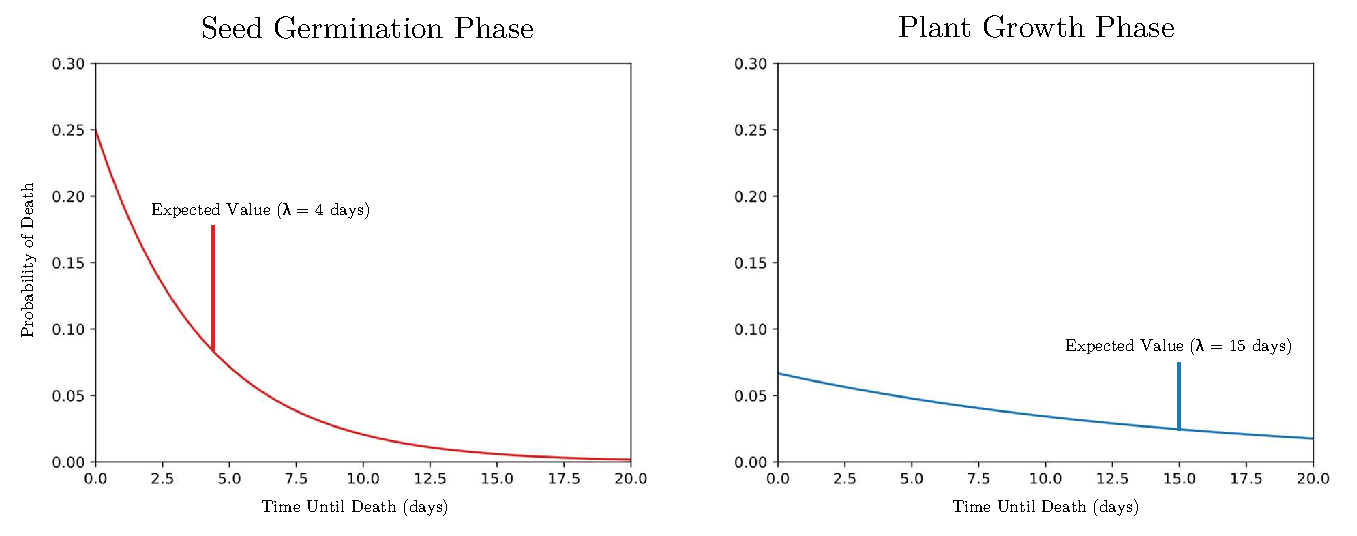
\includegraphics[scale=0.70]{figures/exponentialdistribution.pdf}
    \captionsetup{width=0.9\textwidth}
    \caption{\textbf{The survival rate of a seed during two major phases.}}
    \label{fig:exponentialdistribution}
\end{figure}

%%% ASSIGN DEATH TIME PREMATURELY (ONLY SURVIVE IF IT GERMINATES/pollen before death time)
\subsection{Stages of Dandelion Growth}

During after a dandelion has landed in the ground and a death date has been assigned, we begin to model the dandelion growth process. There are two steps: (phase 1) seed germination and (phase 2) the plant growth process.

Because the seed germination stage is relatively short compared to the much longer plant-growth process, we use historical data to determine a germination length and a longer model to model the plant development cycle (cite data).


\subsubsection{Phase 1: Seed Germination}

To obtain the time for a seed to germinate, we sample from a Normal distribution with parameters \(\mu_{\text{germination}}(t)\) and \(\sigma^2\) with a varying mean time of seed germination based on the climate of the year and region (CITE!).

After every seed germination, we re-sample a probability of death from the seed survival distribution above with a new hazard function \(\lambda_d(t)\) for growing dandelions. This is due to the fact that seeds usually have different expected lifespans compared to dandelion plants, therefore, we assign a \textit{new death date} when a seed finishes its germination process.


\subsubsection{Phase 2: Plant Development}

Once germinated, we define the growth function \(G: [T_I, L_I, N_I] \longrightarrow [0, 1]\) based on three indices \(T_I\), \(L_I\), and \(N_I\) for temperature \(\tau(t)\), light levels \(l(t)\), and soil nutrient composition, respectively. When growth \(G\) is at 0, we say that a single dandelion just began growing (or was just germinated). When the growth \(G\) is at 1, we say that the dandelion is at the "puffball" stage and releases its seeds.

\begin{quote}
\textbf{Temperature Index}

For the \textit{temperature index} \(T_I: \tau(t) \longrightarrow [-1, 1]\), we define a piecewise function where it assigns a negative score if the temperature \(\tau(t)\) in Fahrenheit falls out of the ideal dandelion growth temperatures (\([50,  77]\)) (CITE!) based on a logistic curve and a positive score within based on squared Euclidean distance from optimal. This would allow us to properly scale scores between 0 and 1, while adding a non-linearity factor to weigh the optimal values more heavily. So, we can define \(T_I\) as
\begin{align}
    T_I = 
    \begin{cases}
        \frac{-2}{1+e^{-0.1(\tau(t)-77)}} + 1, \hspace{2cm} & \tau(t) \geq 77 \\
        1 - \frac{1}{63.5^2} (\tau(t) - 63.5), & 50 < \tau(t) < 77 \\
        \frac{-2}{1+e^{-0.1(50-\tau(t))}} + 1, \hspace{2cm} & \tau(t) \leq 50\\
    \end{cases}
\end{align}

%% TALK ABOUT L_I, N_I

\textbf{Light Index}

For the \textit{light index} \(L_I: l(t) \longrightarrow [-1, 1]\), we again define a piecewise function which similarly assigns scores to the temperature index but for the interval of light hours \([6, 24]\). So, we define \(L_I\) as,

\begin{align}
    L_I = 
    \begin{cases}
        \frac{-2}{1+e^{-0.5(l(t)-24)}} + 1, \hspace{2cm} & l(t) \geq 24 \\
        1 - \frac{1}{15^2} (l(t) - 15), & 6 < l(t) < 24 \\
        \frac{-2}{1+e^{-0.5(6-l(t))}} + 1, \hspace{2cm} & l(t) \leq 24 \\
    \end{cases}
\end{align}

\textbf{Nutrition Index}

Lastly, we define the soil \textit{nutrition index} \(N_I: (k(t),n(t)) \longrightarrow [-1, 1]\) to be a function on potassium levels and nitrogen levels (See Assumption~\ref{assumption:5}) in a given region where potassium and nitrogen levels are optimally between \([40, 80]\) and \([20, 40]\) ppm, respectively (CITE!). Based on this information, we formulate the following exponential transformation for the soil nutrient index. By defining a similar shape to the previous index functions and min-max scaling \(k(t)\) and \(n(t)\), we arrive at the following index function.

\begin{align}
    N_I = \exp\left(-\left(\frac{k(t)-60}{40}\right)^2\right) + \exp\left(-\left(\frac{n(t)-30}{30}\right)^2\right) - 1
\end{align}
\end{quote}


Using the three indices above, we  formulate the change in growth, \(\frac{dG(}{dt}(t)\) at time step \(t\) by scaling the sum of \(T_I\), \(L_I\), and \(N_I\) to match the time to fully grow a dandelion under optimal conditions (50 days) (CITE!!). Furthermore, we scale the sum of the indices by \(\frac{1}{3\cdot50}\) as optimal growing conditions would result in \(\frac{dG}{dt} = \frac{1}{50}\). Therefore, we define \(\frac{dG}{dt}(t)\) as,

\begin{align}
    \frac{dG}{dt}(t) = \frac{1}{150}\left(T_I+L_I+N_I\right) \\
    \text{where } \max\left(\frac{dG}{dt}\right) = \frac{1}{50} \nonumber
\end{align}

%%% INSERT FIGURE WITH SHAPE OF EACH

Note that each seed independently begins its growth process after germination. When each seed grows into a fully-fledged plant (\(G = 1\)), it is labeled as its puffball phase. 


\begin{figure}[h!]
\centering
    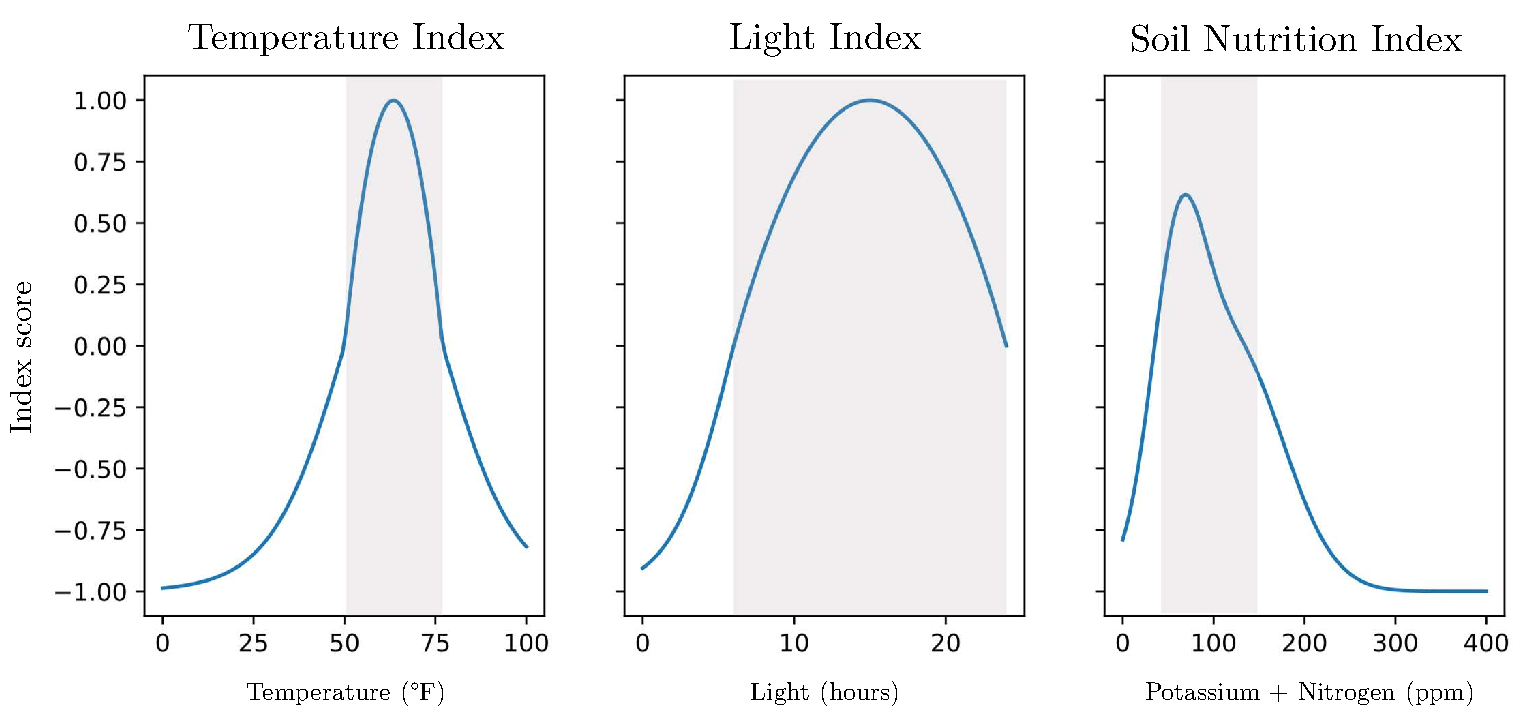
\includegraphics[scale=0.5]{figures/scoreindex.pdf}
    \captionsetup{width=0.9\textwidth}
    \caption{\textbf{From the left to right: \(T_I, L_I, N_I\) scores for plant growth.} Each shaded area represents the optimal interval for each unit of measure, which receives a positive score when within such interval.}
    \label{fig:indexscoregraphs}
\end{figure}

\subsection{Seed Agent Model Overview}

Our method of modeling the spread of dandelions from an agent-based perspective is summarized in Figure~\ref{fig:partadiagram}.

\begin{figure}[h!]
\centering
    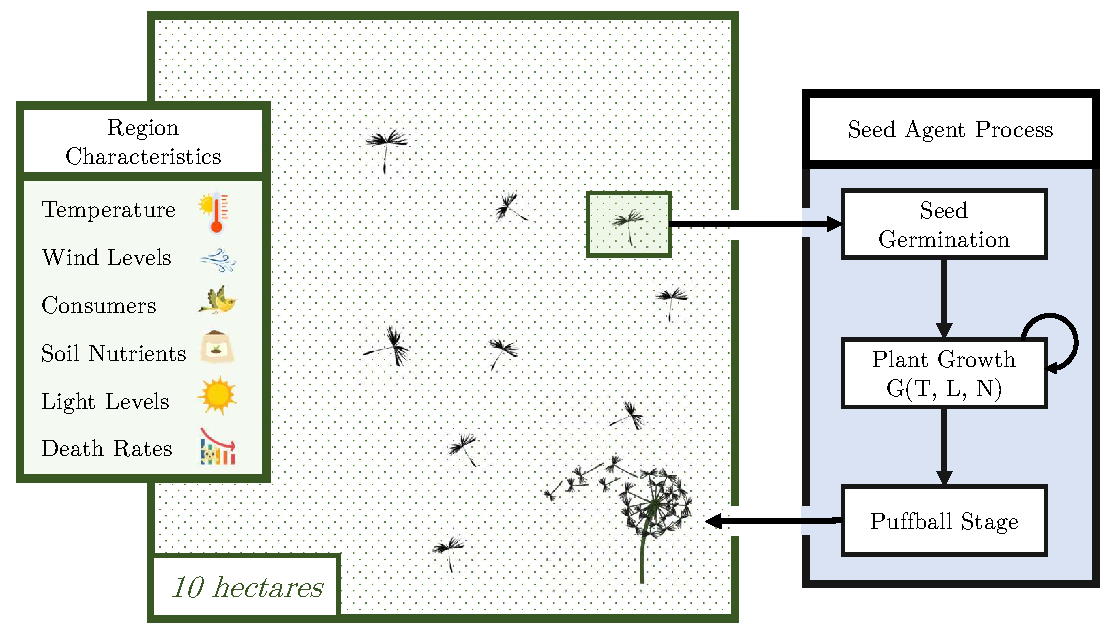
\includegraphics[scale=0.8]{figures/seedspreadprocess2.pdf}
    \captionsetup{width=0.9\textwidth}
    \caption{\textbf{Overview diagram of seed spread modeling.} }
    \label{fig:partadiagram}
\end{figure}